\documentclass[ncrna,article,submit,moreauthors,pdftex,10pt,a4paper]{mdpi} 
\usepackage{color}
\newcommand{\TODO}[1]{\begingroup\color{red}#1\endgroup}
%=================================================================
\firstpage{1} 
\makeatletter 
\setcounter{page}{\@firstpage} 
\makeatother 
\articlenumber{x}
\doinum{10.3390/------}
\pubvolume{xx}
\pubyear{2016}
\copyrightyear{2016}
\externaleditor{Academic Editor: name}
\history{Received: date; Accepted: date; Published: date}
\history{ }
%=================================================================
\Title{Rare Splice Variants in Long Non-Coding RNAs}

\Author{Rituparno Sen$^{1}$, Gero Doose$^{2}$, 
   Peter F. Stadler$^{2-8}$*}

% Authors, for metadata in PDF
\AuthorNames{Rituparno Sen, Gero Doose, Peter F. Stadler}

\address{%
  $^{1}$Bioinformatics Group, Dept.\ Computer Science, and
  Interdisciplinary Center for Bioinformatics, University Leipzig,
  H{\"a}rtelstrasse 16-18, D-04107 Leipzig, Germany\\
  $^{2}$ecSeq Bioinformatics, Brandvorwerkstra{\ss}e 43,
  D-04275 Leipzig, Germany\\
  $^{3}$German Centre for Integrative Biodiversity Research (iDiv)
  Halle-Jena-Leipzig, Competence Center for Scalable Data Services and
  Solutions; Leipzig Research Center for Civilization Diseases; and Leipzig
  Research Center for Civilization Diseases (LIFE), University Leipzig\\
  $^{4}$Max Planck Institute for Mathematics in the Sciences,
  Inselstra{\ss}e 22, D-04103 Leipzig, Germany\\
  $^{5}$Fraunhofer Institute for Cell Therapy and Immunology,
  Perlickstrasse 1, D-04103 Leipzig, Germany\\
  $^{6}$Center for RNA in Technology and Health, Univ. Copenhagen,
  Gr{\o}nneg{\aa}rdsvej 3, Frederiksberg C, Denmark\\
  $^{7}$Santa Fe Institute, 1399 Hyde Park Road, Santa Fe NM 87501, USA }

\corres{Correspondence: studla@bioinf.uni-leipzig.de; Tel.: +49 341 97-16690}

\abstract{Long noncoding RNAs(lncRNAs) are constantly being discovered and
  we are in a nascent stage of understanding their sequence structure. We
  performed statistical analyses on exon and intron content of lncRNA
  annotation data from different publicly available annotation datasets.
  We have used sophisticated alignment algorithms as well as custom
  analysis scripts to investigate the transcriptomic structure of lncRNAs.}

\keyword{\TODO{keywords}}

\begin{document}

\section{Introduction}

lncRNAs are of growing interest, furthermore novel lncRNA genes play key functional roles in important biological processes.
Many lncRNA transcripts act as potential regulators in cellular functionalities. One of the well known functions of lncRNAs is 
in gene silencing through interaction with chromatin [Cite Guttman, 2012]. lncRNA HULC[Cite Tay, 2014] has been detected to be over expressed in hepatocellular carcinoma. ANRIL 
In recent years increasing number of researchers have focused on the annotation landscape of the lncRNAs.

The Ensembl project [Cite Hubbard, 2001] aims to assemble biological data and present it to researchers. The human genome annotation data contains known genes
and also predicted novel genes. Each dataset contains transcriptomic information with genes, transcripts and number of exons for every transcript.

GENCODE[Cite Harrow, 2012] is an annotation dataset which provides information about protein coding loci as well as long noncoding gene loci in the human genome. 
It presents a combination of manual and automated annotation techniques which endeavours to list gene features from HAVANA and Ensembl datasets.
It categorises the data through various attributes such as the gene locus, the number of transcripts, the number of exons per transcript, 
the biotypes of the lncRNAs.

A research carried out by Cabili et al[Cite Cabili, 2011] catalogues long intergenic noncoding RNAs(lincRNAs) with reads across 24 tissues. More than 30 characteristic features 
are chosen from high throughput RNA Seq data as well as available annotation datasets to functionally classify the lincRNA genes.

The latest version of the NONCODE database [Cite Zhao, 2015] contains annotation data of noncoding RNAs of 16 species. This database provides conservation 
information of the lncRNAs, along with how the lncRNAs are related to various diseases.\\

However, despite much focus on the proper annotation of the lncRNA genes, a few questions about the splice sites remain unanswered. lncRNAs, unlike mRNAs,
do not undergo translation, but they are spliced and can possess multiple isoforms. In this paper, we attempt to illustrate the presence of 
splice sites which are not hitherto revealed. 




\section{Results}

In this project, we sought to investigate the annotation landscape of lncRNAs and identify any unrevealed splice sites present
in any gene loci.
It is evident from the results there are a few novel exons present in the gene model reported by the GENCODE authors. As can be observed in
Fig \ref{F03} and Fig \ref{F04}, clearly there are novel exons present which were not included/detected in the gene model.
\begin{figure}[h]
 \subfigure[Fig. 5]{\label{F05}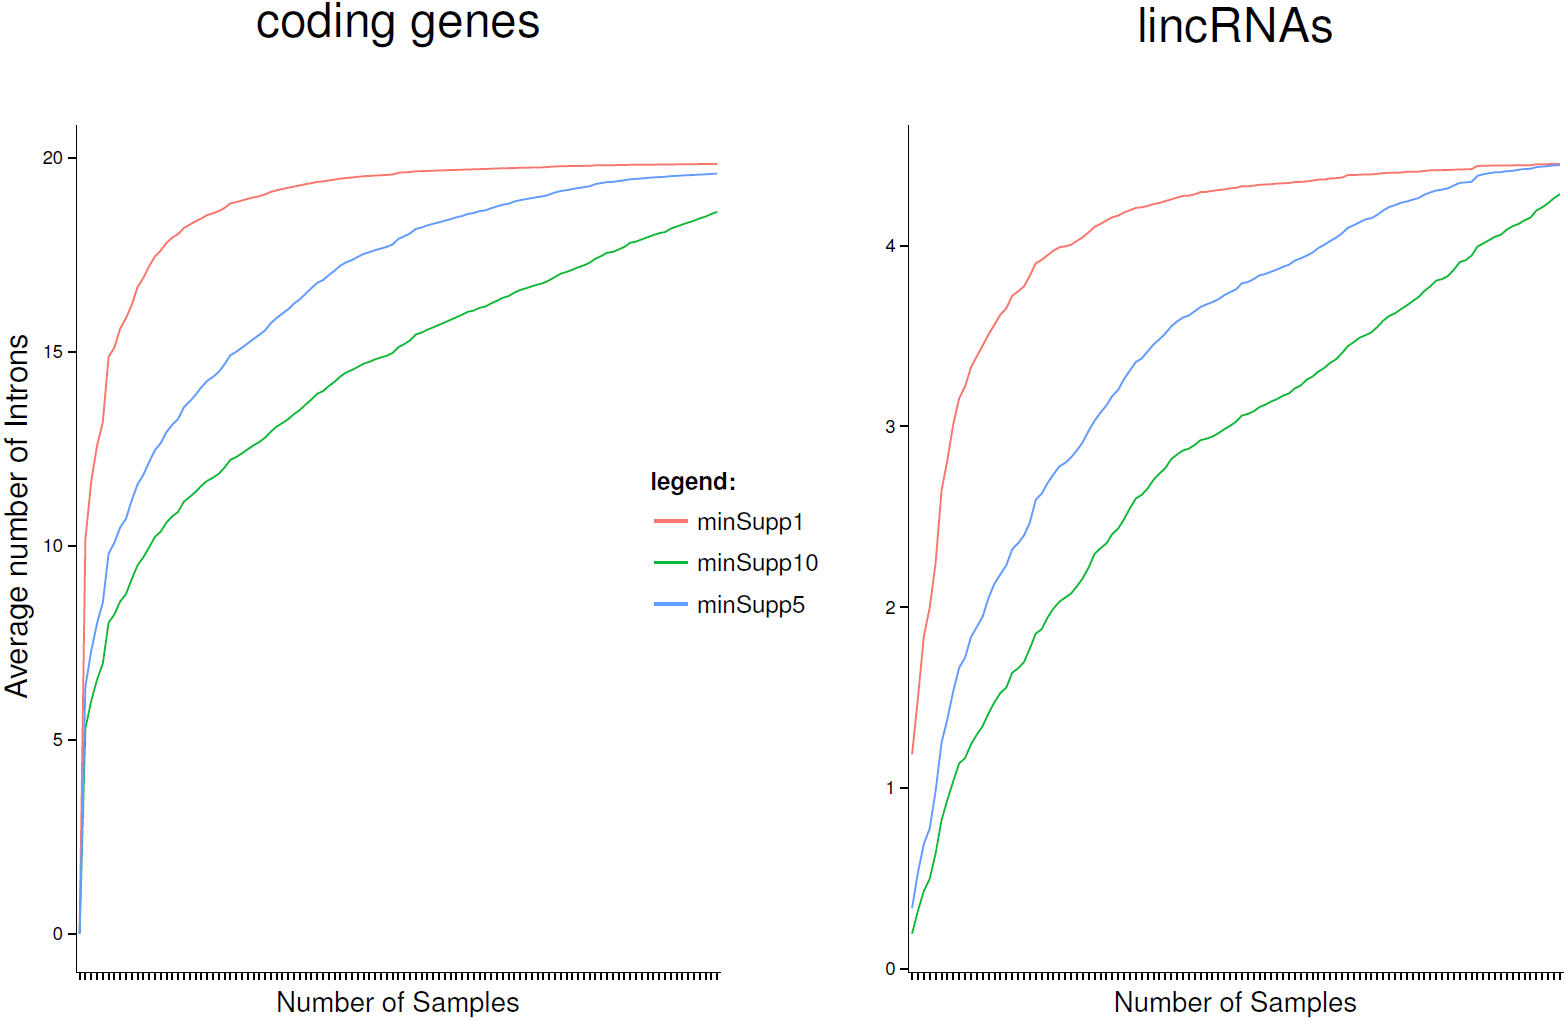
\includegraphics[width=\linewidth]{/homes/biertruck/rituparno/Documents/Raw/fig1.png}}
 \subfigure[Fig. 6]{\label{F06}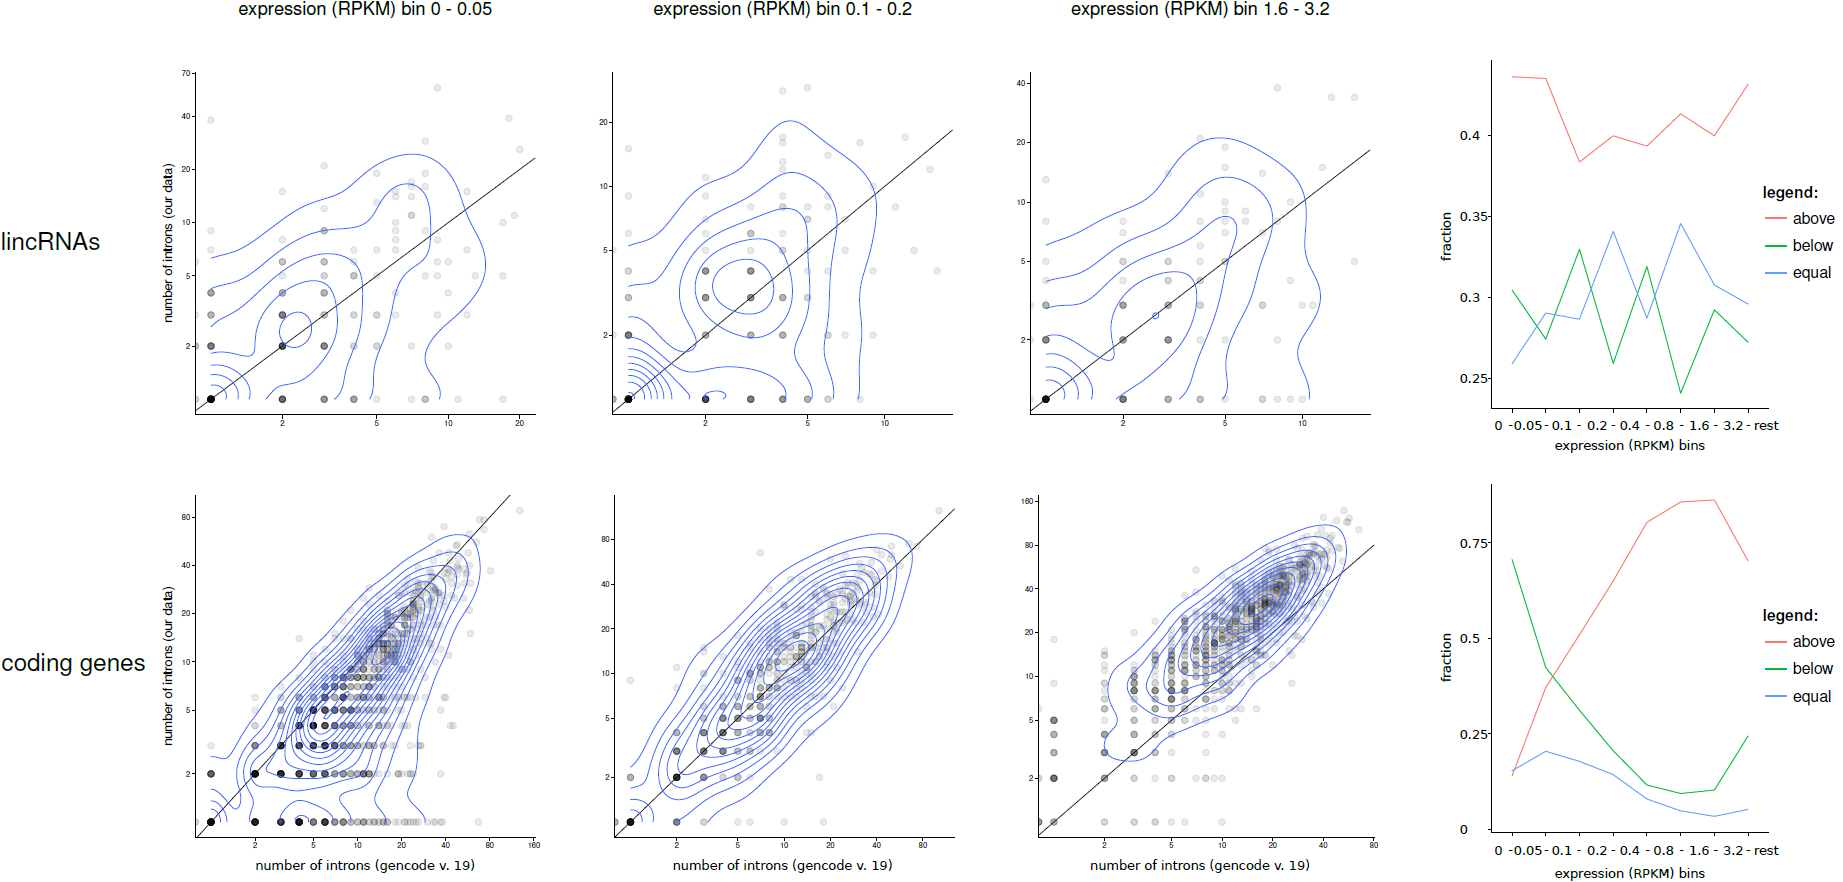
\includegraphics[width=\linewidth, height=8cm]{/homes/biertruck/rituparno/Documents/Raw/fig2.png}}
\end{figure}

%edit these plots. replot, manipulate in Inkscape.
\begin{figure}[ht]
 \centering 
 \subfigure[]
 {\includegraphics[width=\linewidth]{/homes/biertruck/rituparno/Documents/Raw/Gencode_v24.png}}
 \label{F07}
 \subfigure[These two plots show the frequency of occurence of exons and introns against transcripts in GENCODE versions 7 and 24]
 {\includegraphics[width=\linewidth]{/homes/biertruck/rituparno/Documents/Raw/Gencode_v7.pdf}}
 \label{F08}
\end{figure}

%\bibliography{abbr_long,references}
\section{Discussion}


\section{Conclusions}

\section{Materials and Methods}

To analyse the annotation landscape of lncRNAs, the whole transcriptome sequencing data from GENCODE, Ensembl, NONCODE 2016, 
and the dataset from Cabili et. al. were used. GENCODE versions from 7 through 24 were used, as well as Ensembl 54 and 83.
The contents of the datasets are laid out in broadly three categories: the location of the lncRNA gene in the locus, 
the transcripts, and the exon locations within the transcripts. One of the primary aims was to calculate
the number of unique introns in each dataset. 

It is known that, an individual gene can contain multiple transcripts, resulting in the presence of common exons among the transcripts.
 Consequently, a pipeline was created to calculate the unique number of exons present in every gene for every version of each dataset. 
 Each dataset was carefully parsed and filtered to obtain calculate the number of exons present using a simple algorithm. Subsequently
 the presence of introns were also accounted for.
 
 \paragraph{}
 The in house transcriptomic data from different types of cancer (viz. follicular lymphoma, B-cell lymphoma) yielded a lot of lncRNAs. 
 The genes available to us were taken from GENCODE v19.
 They were mapped against all the versions of the GENCODE datasets to obtain a count of the exonic and intronic content. 
  On mapping them against v7 and v24, we found that close to 60\% of the genes
 were calculated in v7 and around 95\% in v24(Table 2). The means of exons and introns are significantly lower than in GENCODE. 

% latex table generated in R 3.3.1 by xtable 1.7-4 package
% \begin{table}[ht]
% \centering
% {\tiny
% \begin{tabular}{p{2cm}|p{0.04\textwidth}p{0.04\textwidth}p{0.04\textwidth}p{0.04\textwidth}p{0.04\textwidth}p{0.04\textwidth}p{0.04\textwidth}p{0.04\textwidth}}
%   \hline
% X & Genes & Transcripts & Exons & Mean.of.Exons & Median.of.Exons & Introns & Mean.of.Introns & Median.of.Introns \\ 
%   \hline
% Ensembl 83 & 9597 & 14038 & 42819 & 3.05 &   3 & 28781 & 2.05 &   2 \\ 
%   Ensembl 54 & 15710 & 26799 & 67583 & 2.52 &   3 & 51877 & 1.94 &   2 \\ 
%   Cabili 2011 & 8263 & 14353 & 33045 & 2.30 &   2 & 18607 & 1.30 &   1 \\ 
%   NONCODE 2016 & 160376 & 233696 & 536111 & 2.29 &   2 & 305771 & 1.31 &   1 \\ 
%   GENCODE v7 & 9580 & 14984 & 42060 & 2.81 &   3 & 28998 & 1.94 &   2 \\ 
%   GENCODE v24 & 15941 & 28031 & 68457 & 2.44 &   2 & 45016 & 1.61 &   1 \\ 
%    \hline
% \end{tabular}
% }
% \caption{All Consortia} 
% \label{tab:01}
% \end{table}


% Tue Aug 16 20:01:50 2016
\begin{table}[ht]
\caption{All Consortia} 
\centering
{\tiny
\begin{tabular}[lrrrrrrrr]{p{0.11\textwidth}|p{0.04\textwidth}p{0.07\textwidth}p{0.04\textwidth}p{0.09\textwidth}
p{0.09\textwidth}p{0.04\textwidth}p{0.11\textwidth}p{0.09\textwidth}}
  \hline
 & Genes & Transcripts & Exons & Mean of Exons & Median of Exons & Introns & Mean of Introns & Median of Introns \\ 
   \hline
Ensembl 83 & 9597 & 14038 & 42819 & 3.05 &   3 & 28781 & 2.05 &   2 \\ 
  Ensembl 54 & 15710 & 26799 & 67583 & 2.52 &   3 & 51877 & 1.94 &   2 \\ 
  Cabili 2011 & 8263 & 14353 & 33045 & 2.30 &   2 & 18607 & 1.30 &   1 \\ 
  NONCODE 2016 & 160376 & 233696 & 536111 & 2.29 &   2 & 305771 & 1.31 &   1 \\ 
  GENCODE v7 & 9580 & 14984 & 42060 & 2.81 &   3 & 28998 & 1.94 &   2 \\ 
  GENCODE v24 & 15941 & 28031 & 68457 & 2.44 &   2 & 45016 & 1.61 &   1 \\ 
   \hline
\end{tabular}
}
\end{table}% latex table generated in R 3.3.1 by xtable 1.7-4 package


\begin{table}[ht]
\centering
{\tiny
\begin{tabular}[lrrrrrrrr]{p{0.11\textwidth}|p{0.04\textwidth}p{0.07\textwidth}p{0.04\textwidth}p{0.09\textwidth}
p{0.09\textwidth}p{0.04\textwidth}p{0.11\textwidth}p{0.09\textwidth}}
  \hline
 & Genes & Transcripts & Exons & Mean of Exons & Median of Exons & Introns & Mean of Introns & Median of Introns \\ 
   \hline
v7 & 3296 & 4563 & 12584 & 2.76 & 3 & 8394 & 1.84 & 2\\
  v19 & 5257 & 7487 & 18774 & 2.51 & 2 & 12010 & 1.6\\
  v24 & 4961 & 7318 & 18685 & 2.55 & 3 & 12202 & 1.67 & 1\\ 
   \hline
\end{tabular}
}
\caption{Our data against the number of genes that were found in GENCODE} 
\end{table}% latex table generated in R 3.3.1 by xtable 1.7-4 package
\newpage


The GENCODE v7 dataset categorises the lncRNA transcripts as antisense, lincRNA, processed\_transcript and sense\_intronic biotypes. 

The authors reported 9640 lncRNA genes with 15, 512 transcripts and the mean of exons per lncRNA transcript is 2.
Whereas using the same set of genes as can be found in the v7 dataset, 9580 genes with 14984 transcripts were identified in this analysis, although 
the mean of exons per lncRNA transcript was identically computed to be 2.
\begin{figure}[hl]
% \subfigure[Com]\includegraphics[width=3cm, height=4cm]{/homes/biertruck/rituparno/Documents/Raw/comarison_plot_2.pdf}
 \subfigure[Plot to compare the distribution of introns in lncRNA genes in our dataset against GENCODE v19]
 {\label{F01}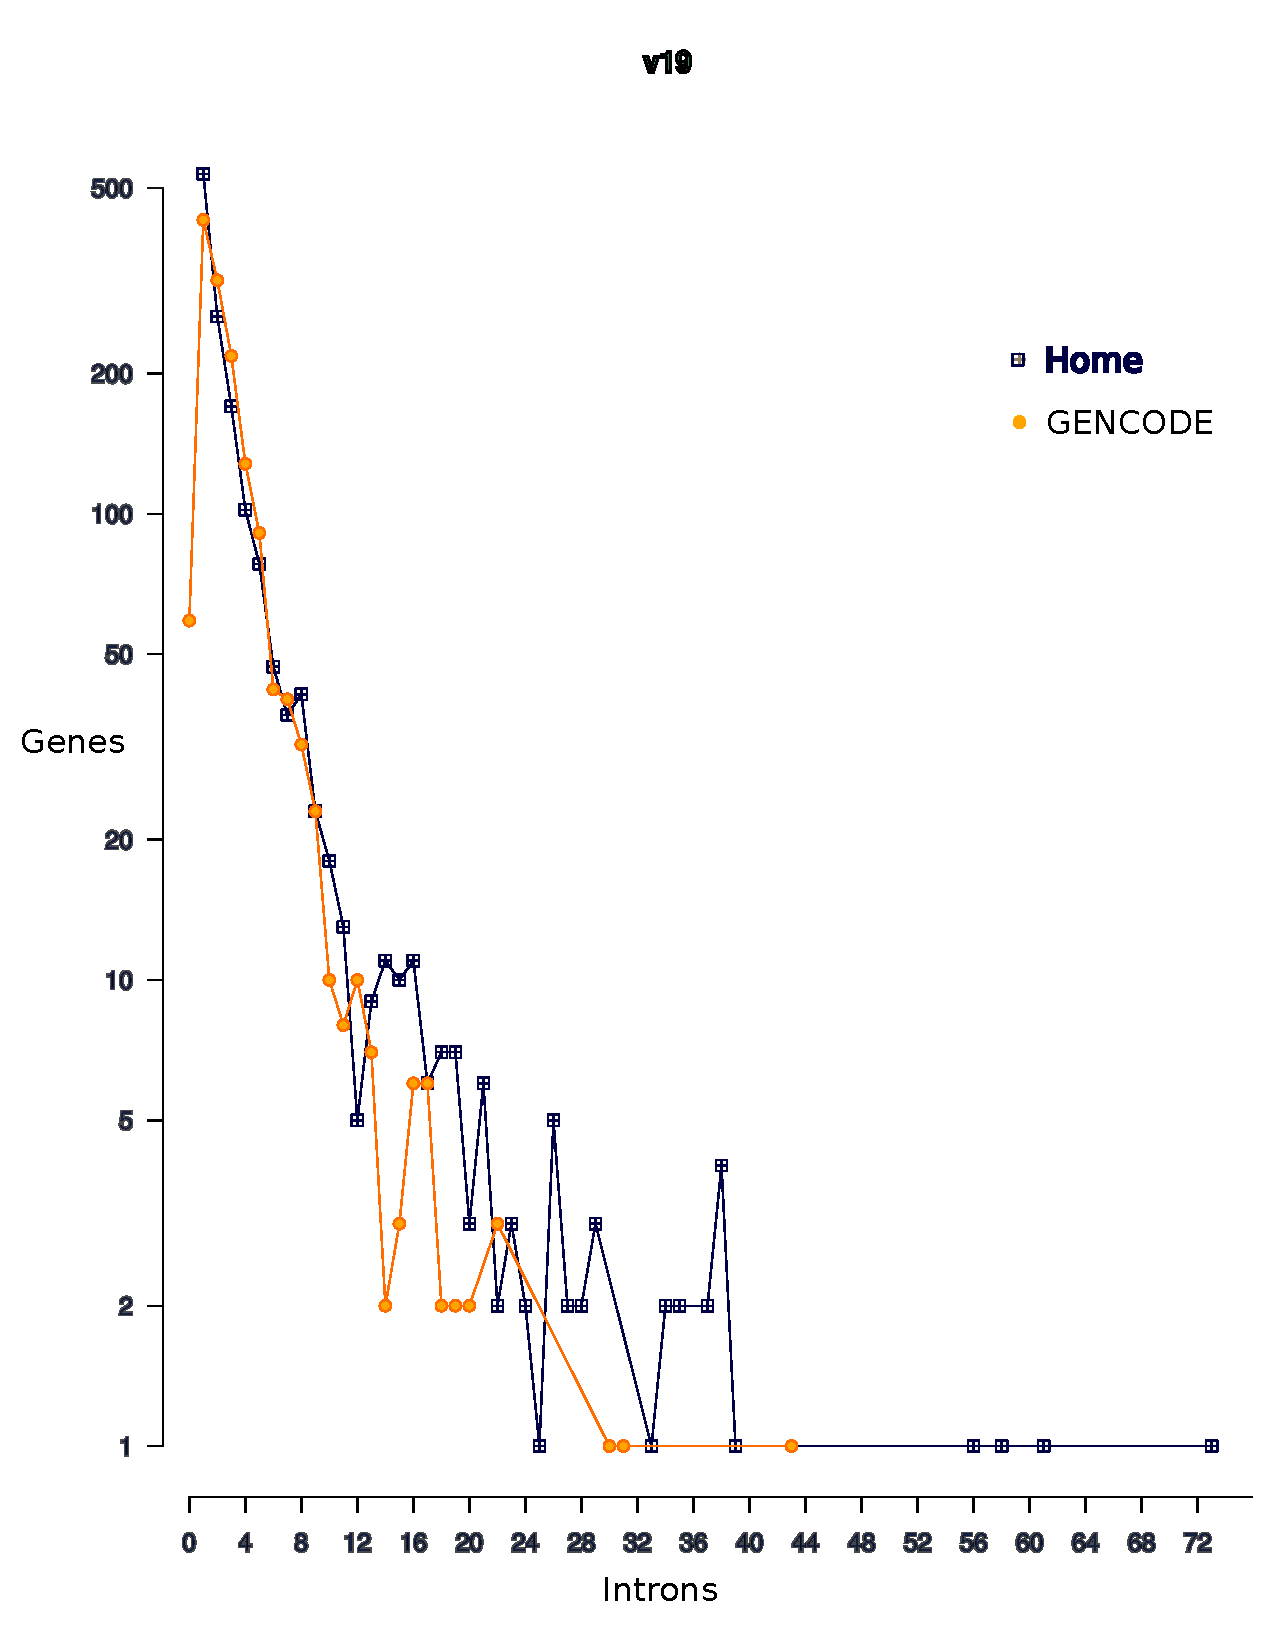
\includegraphics[width=\textwidth, height=12cm]{/homes/biertruck/rituparno/Documents/Raw/comparison_plot_2.pdf}}
\end{figure}
\begin{figure}[hl]
 \centering
 \subfigure[This boxplot shows that the number of introns in our dataset is more than that found in GENCODE v19, although the mean remains similar]
 {\label{F02}\includegraphics[width=0.8\linewidth]{/homes/biertruck/rituparno/Documents/Raw/boxplot_both_1.pdf}}
\end{figure}

The current analysis was conducted primarily based on GENCODE datasets from versions 7 through 24. 
The datasets are provided in the standard GTF format. Every dataset classifies a gene with a variety of characteristics, including
the exact locations of genes, their transcripts, and the transcripts contain. As the locations of transcripts overlap in a
gene locus, thus allowing exons to be shared among the transcripts.
Using custom scripts the number of unique exons present in every gene was determined, which also permitted the calculation
of the number of unique introns per gene. Moreover, the number of transcripts for every biotype was also documented.
Furthermore, the mean and median of exons and introns for each dataset was also computed.
\begin{figure}[hl]
 \subfigure[For the lncRNA gene ENSG00000267939 GENCODE v19 reported one intron. Our analysis resulted in the presence of 6 introns with two potential exons]
 {\label{F03}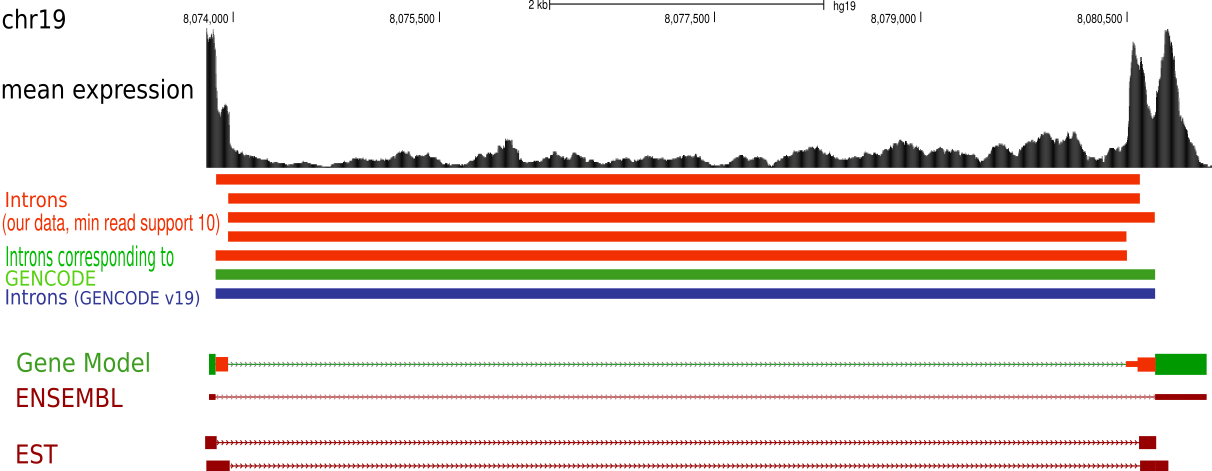
\includegraphics[width=\linewidth]{/homes/biertruck/rituparno/Documents/Raw/267939.png}}
 \subfigure[GENCODE reported two introns for the gene ENSG00000263470 but we are reporting 9, including one false positive]
 {\label{F04}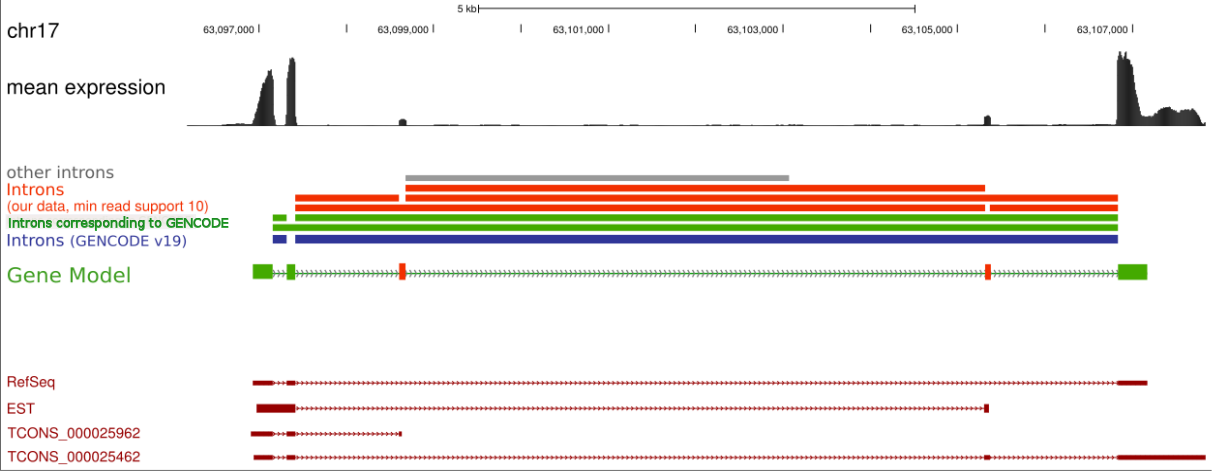
\includegraphics[width=\linewidth]{/homes/biertruck/rituparno/Documents/Raw/example.png}}
\end{figure}
  
In order to analyse the sequence structure in more details on the UCSC Genome Browser, a batch of genes from the sample dataset 
were carefully identified and selected whose intron content was significanty greater than reported in GENCODE v19. A minimum read support of 10
was further applied to optimise the list.
We present two examples here. 
The lncRNA gene ENSG00000267939 has one intron as reported by GENCODE; on the contrary, the same gene was found to have 
6 introns including the one reported. (or 5 novel introns?) There were two potential(novel?) exons. Fig \ref{F03} shows the possibility of 
existence of the exons through the EST strands. Fig \ref{F04} shows the gene ENSG00000263470 which has 3 unique exons and 2 unique introns 
as reported by GENCODE. 
However, in this study 9 unique introns in the gene with a false positive were discovered. There were two novel exons in the gene model 
which was consolidated by the EST and TCONS data.


%%%%%%%%%%%%%%%%%%%%%%%%%%%%%%%%%%%%%%%%%%
\vspace{6pt} 

%%%%%%%%%%%%%%%%%%%%%%%%%%%%%%%%%%%%%%%%%%
%% optional
\supplementary{
The following are available online at www.mdpi.com/link, Figure S1: title, Table S1: title, Video S1: title.}

%%%%%%%%%%%%%%%%%%%%%%%%%%%%%%%%%%%%%%%%%%
\acknowledgments{\TODO{Ritu DAAD grant}}}

%%%%%%%%%%%%%%%%%%%%%%%%%%%%%%%%%%%%%%%%%%
\authorcontributions{PFS designed the study, RS and GD analyzed the
  data. All authors contributed to the interpreation of the data and the
  writing of the manuscript.}

%%%%%%%%%%%%%%%%%%%%%%%%%%%%%%%%%%%%%%%%%%
\conflictofinterests{The authors declare no conflict of interest.}

%%%%%%%%%%%%%%%%%%%%%%%%%%%%%%%%%%%%%%%%%%
%% optional
\abbreviations{The following abbreviations are used in this manuscript:\\

\noindent 
\begin{tabular}{@{}ll}
snoRNA & small nucleolar RNA\\
rRNA   & ribosomal RNA
\end{tabular}}

\bibliographystyle{mdpi}
\bibliography{ritu01}

\end{document}

